\documentclass[12pt,prb,aps,epsf]{report}
\usepackage[utf8]{inputenc}
\usepackage{amsmath}
\usepackage{amsfonts}
\usepackage{amssymb}
\usepackage{graphicx} 
\usepackage{latexsym} 
\usepackage[toc,page]{appendix}
\usepackage{listings}
\usepackage{xcolor}
\usepackage{soul}
\usepackage[T1]{fontenc}
\usepackage{amsthm}
\usepackage{mathtools}
\usepackage{setspace}
\usepackage{array,multirow,makecell}
\usepackage{geometry}
\usepackage{textcomp}
\usepackage{float}
\usepackage{cancel}
\usepackage{here}
\usepackage{titlesec}
\usepackage{bbold}

\geometry{hmargin=2cm,vmargin=2cm}

\begin{document}
	
	\title{MP 4 Capteurs de grandeurs mécaniques}
	\author{Sébastien}
	
	\maketitle
	
	\tableofcontents
	
	\pagebreak
	
\section{introduction}
Def capteur
	
\section{La balance électronique : capteur de masse par déformation d'une jauge de contrainte}
\paragraph{Montage :} on impose une contrainte via une masse sur un pont de Winstone (=jauge de contrainte) et on amplifie le signal de sortie en utilisant un amplificateur d'autocomutation. On trace ensuite la tension de sortie en fonction de la masse : $U_s(m)$ avec des masses étalon. Via cette droite d'étalonnage on peut ensuite mesurer une masse inconnue. (comparaison avec résultat donné par une balance commerciale étalon). On calcule ensuite les incertitudes de la mesure avec :
\begin{eqnarray}
S=\frac{\Delta U_s}{\Delta m}\\
m_{mesurée} = \frac{U_{S_{mes}}-U_{min}}{S}\\
\left(\frac{\Delta m}{m}\right)^2 = \left(\frac{\Delta U_{S_{mes}}}{U_{S_{mes}}}\right)^2 + \left(\frac{\Delta S}{S}\right)^2
\end{eqnarray}
Rq: la droite d'étalonnage possède un offset : tension non nulle pour masse nulle.
\section{Détermination de la déformation d'un piézoélectrique par interférométrie}

\begin{figure}[h]
	\centerline{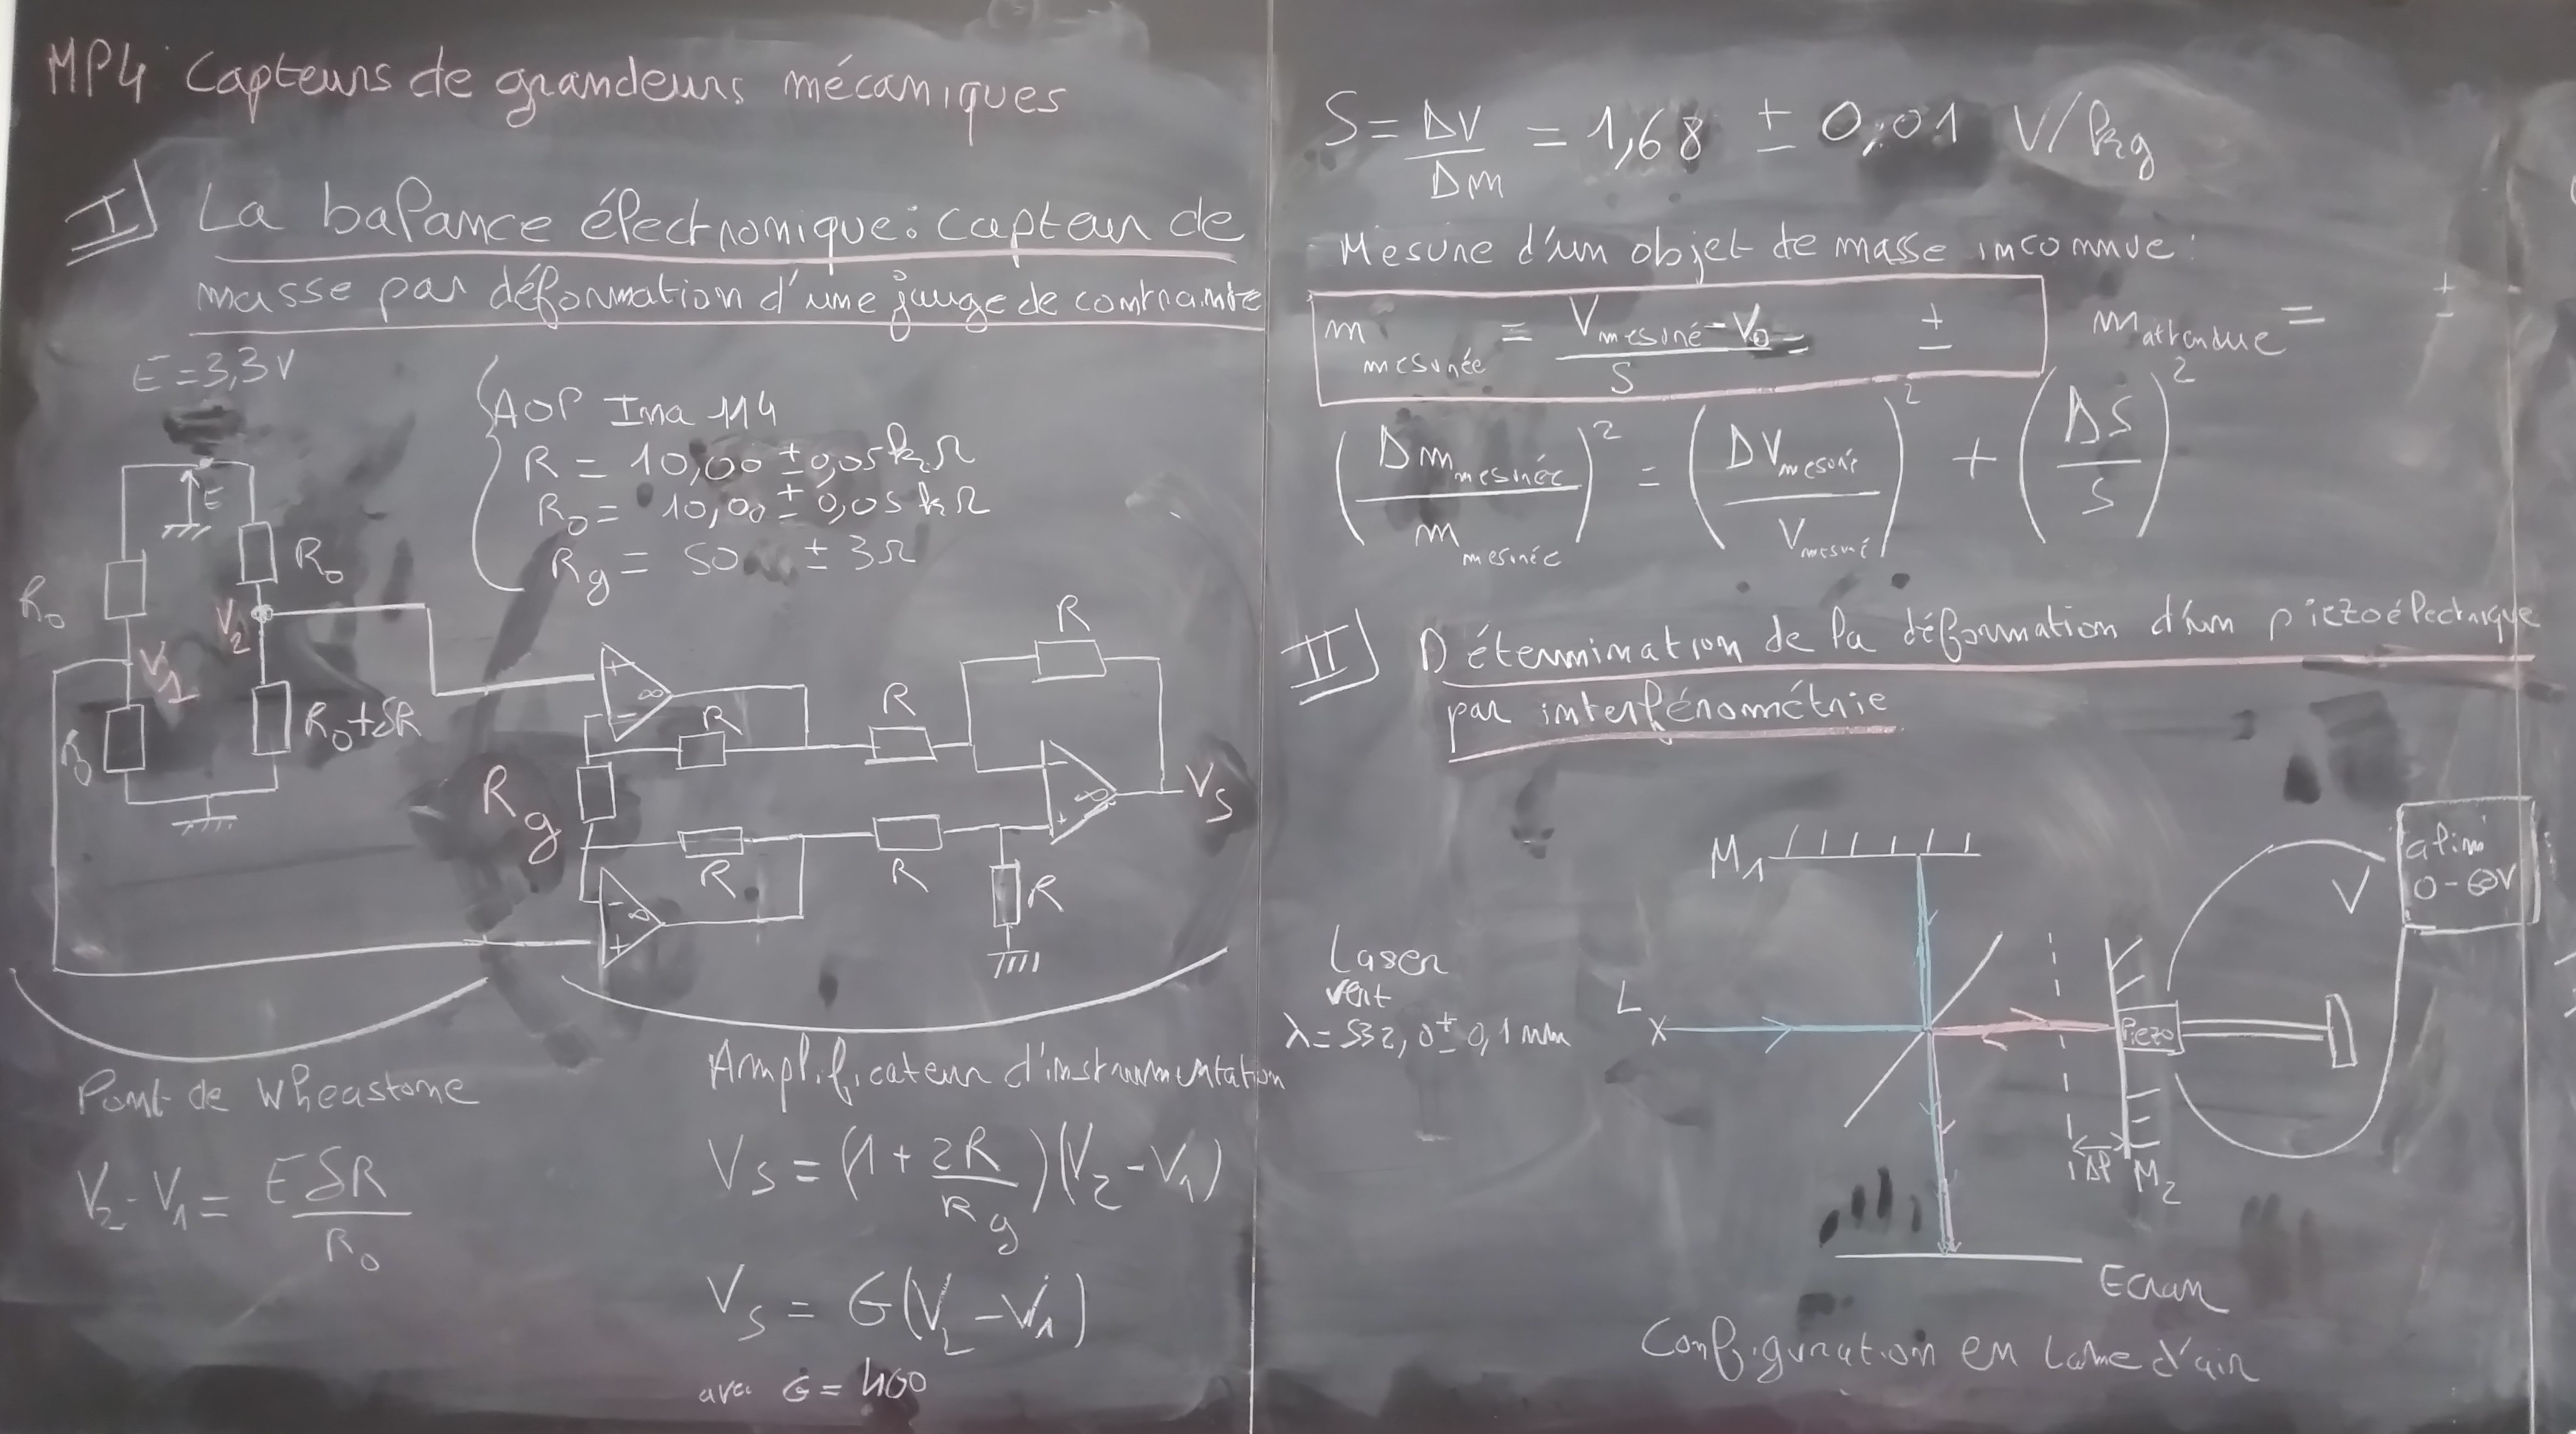
\includegraphics[width=18cm]{P_20181010_095430}}
\end{figure}
On place le michelson près du contact optique grace à un laser, et on compte, pour un votage donné, le nombre de franges "avalées" $n$, ce qui permet de déduire le déplacement généré par le piézo avec 
\begin{eqnarray}
l_{piezo} = n2\lambda_{laser}
\end{eqnarray}
On peut ensuite comparer avec le valeur théorique: 
\begin{eqnarray}
S = \frac{\Delta l}{\Delta V} = 60 +- 12\, nm/V
\end{eqnarray}
\begin{figure}
	\centerline{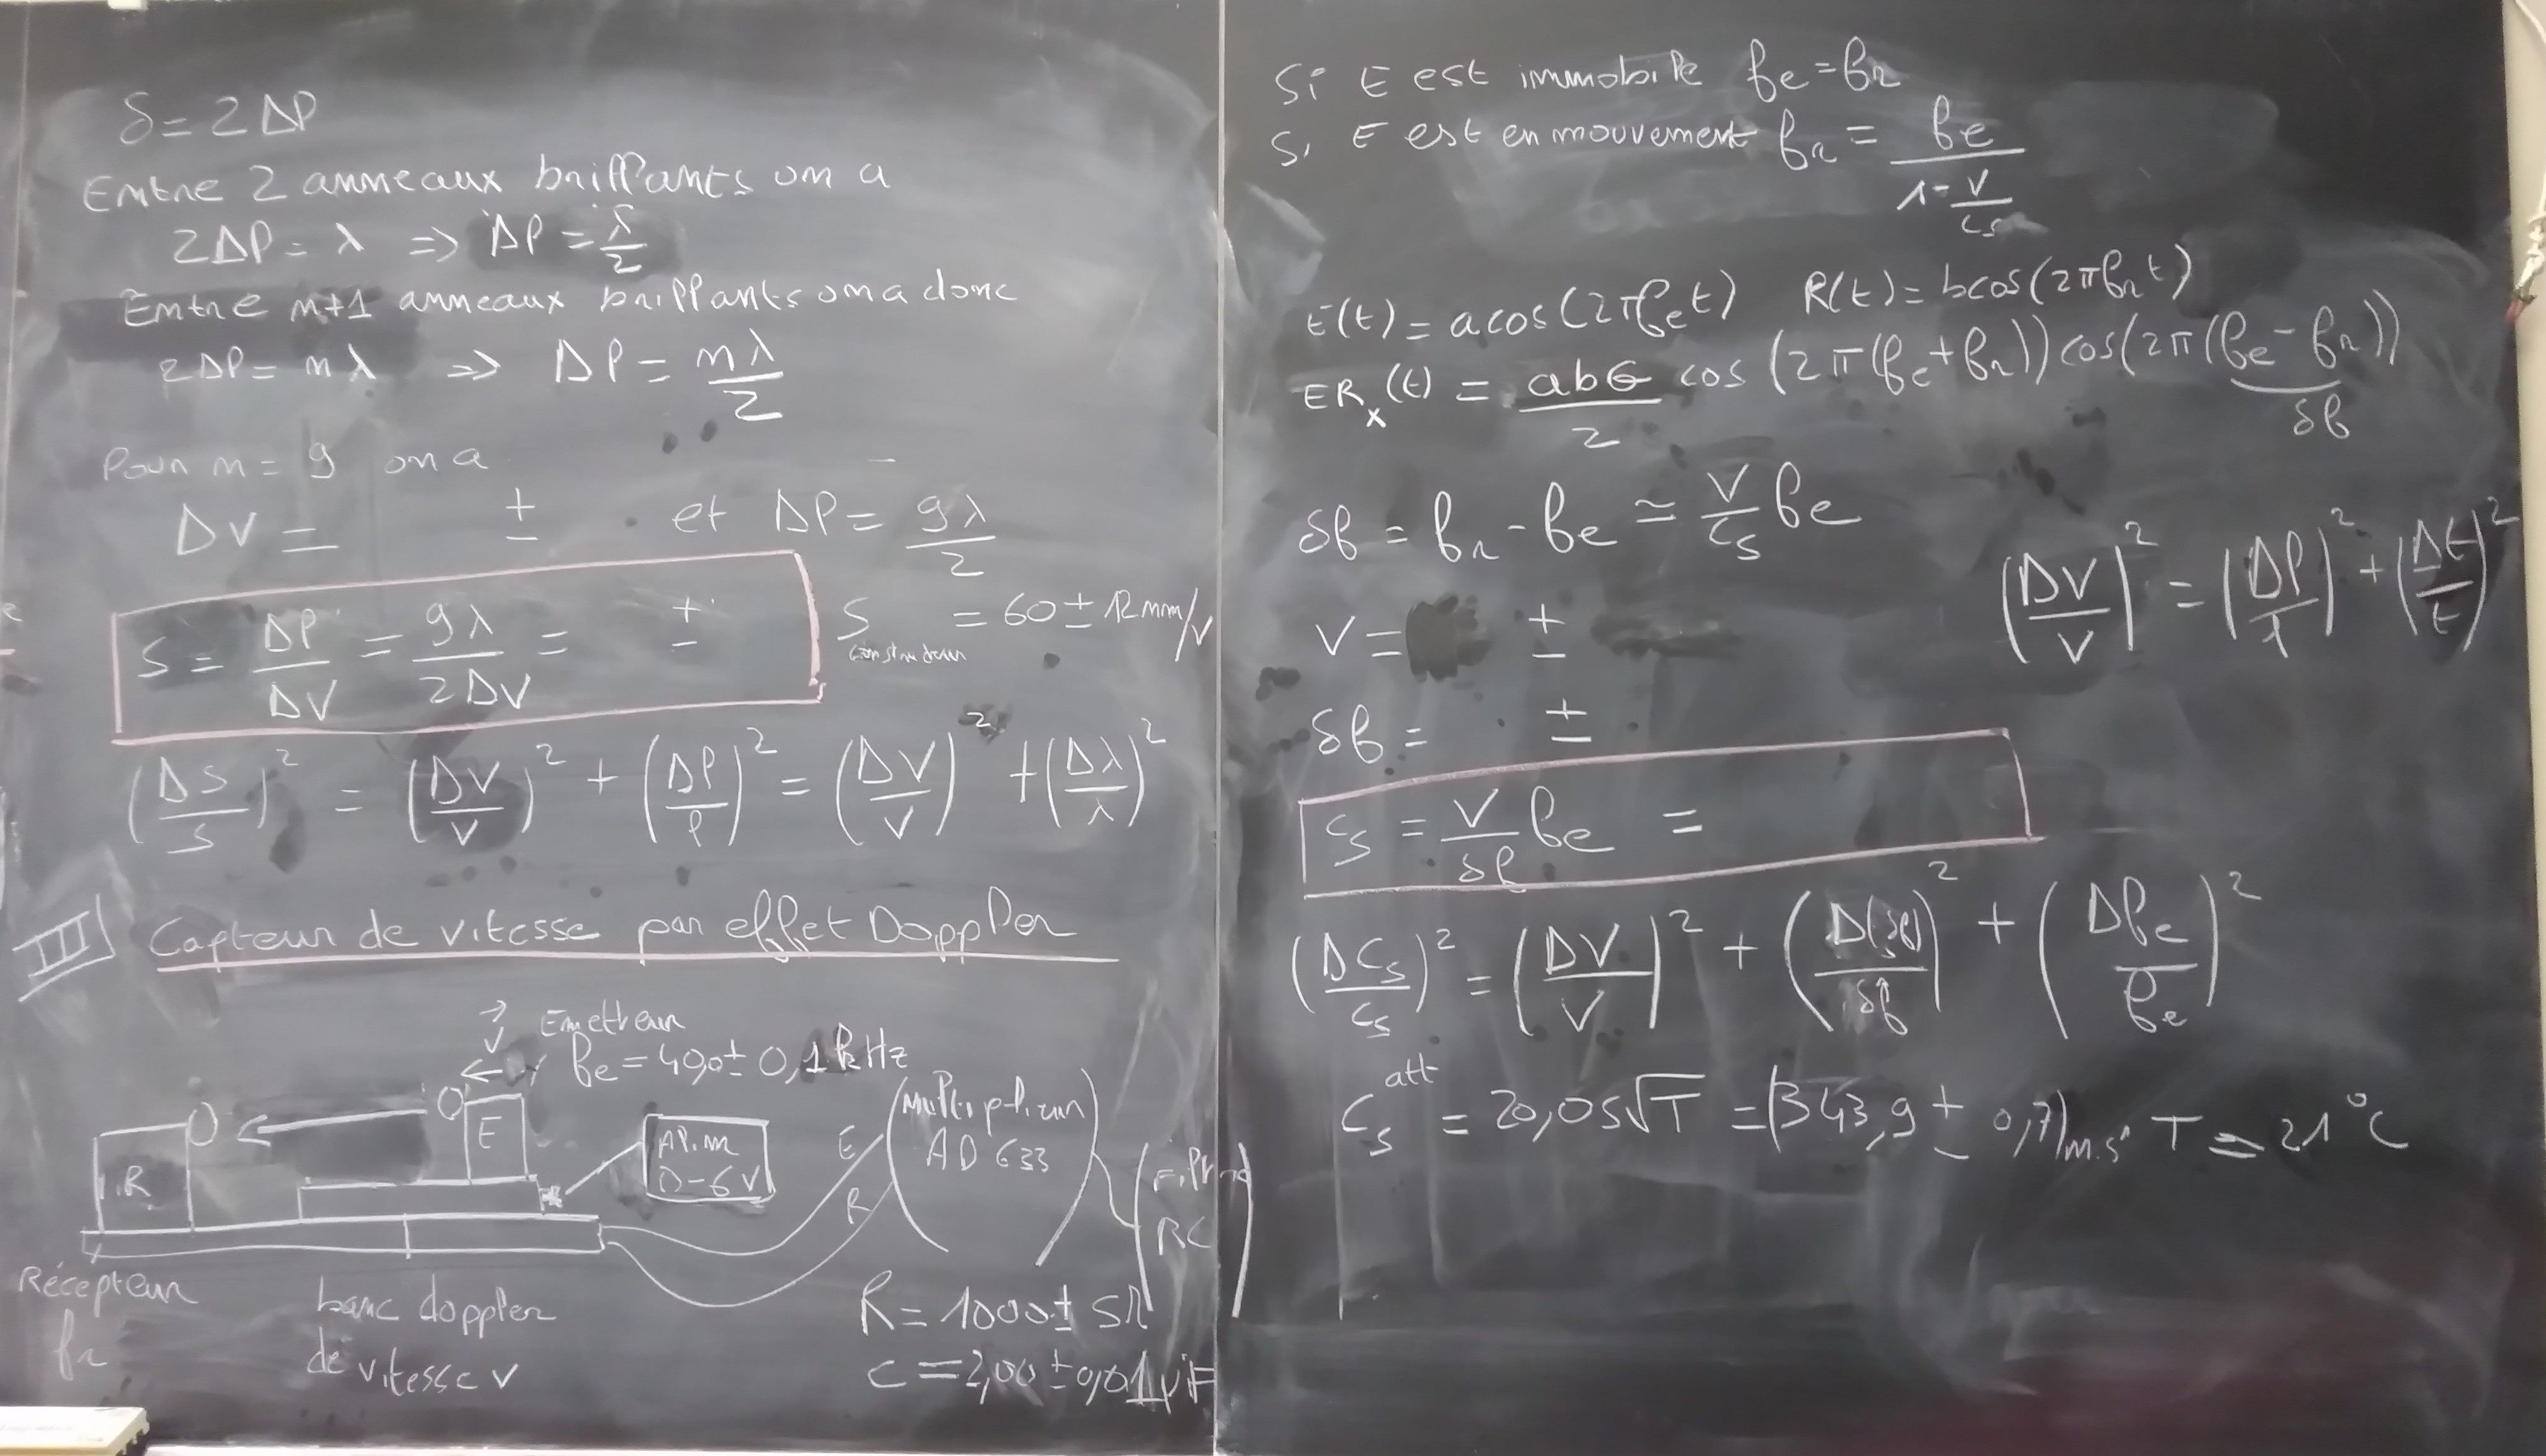
\includegraphics[width=18cm]{P_20181010_095444}}
\end{figure}
\section{Capteur de vitesse par effet Doppler}
On chronomètre pour avoir la vitesse de déplacement du capteur, et on observe dans un même temps la fréquence du signal reçu, par rapport à la fréquence du signal  émis par l'émetteur qui est quand à lui fixe. on obtient ainsi un $\delta f$ fonction de la vitesse, selon 
\begin{eqnarray}
\Delta f = f_r-f_e \simeq \frac{Vf_e}{c_s}
\end{eqnarray} 
où $c_s$ est la vitesse du son. Connaissant V (car on l'a mesurée), on peut en déduire la vitesse du son 
\begin{eqnarray}
c_s = \frac{Vf_e}{\delta f}
\end{eqnarray}
avec l'incertitude relative associée 
\begin{eqnarray}
\left(\frac{\Delta c_s}{c_s}\right)^2 = \left(\frac{\Delta \delta f}{\delta f}\right)^2 + \left(\frac{\Delta f_e}{f_e}\right)^2
\end{eqnarray}




\section{Questions}
Quelles sont les grandeurs mécaniques ??\\
Vitesse, accélération, longueur, masse...\\

Pouvez vous redéfinir la notion de capteur ?\\
Transforme grandeur physique en grandeur électrique.\\

Quelles sont ces grandeurs électriques ?\\
Capacité, tension, inductance, résistance, intensité et 1 de plus\\

Pont de Winstone : quelle est la grandeur physique appliquée à la résistance ? Et comment la résistance varie en fonction de cette grandeur physique (la masse) ?\\
Si la résistance ne varie pas alors la tension est nulle.\\

Utilité de l'amplificateur ? amplifie t-il une différence de tension ou une tension relative à la masse ?\\
Pouvoir mesurer une faible différence de tension associée à une faible masse. Une différence de tension.\\

Pourquoi ce choix d'amplificateur, pourquoi ne pas prendre un ampli "simple" avec 1 seul AOp ?\\
Élimination d'un terme, qui est non constant et donc indésirable.\\

Comment peut on voir si il y a un offset ? Et comment le corriger ?\\
Mesure de $U_s$ pour une masse nulle. En théorie les 4 résistances valent $R_0$ à masse nulle, et il n'y a donc pas d'offset, si ce n'est pas le cas : modif de la valeur de ces résistances.\\

\paragraph{Concernant le graphe $U_s(m)$ :}
Est ce une mesure de sensibilité statique ou dynamique ?\\
Statique.\\
Pourquoi cherche t-on un modèle linéaire ?\\
Concernant la répétabilité, que peut on faire quantitativement de plusieurs séries de mesures ? écart type ? répartition statistique des mesures ?\\

\paragraph{Concernant le capteur de vitesse :} 
Pouvez vous refaire la mesure en directe ? Comment choisir N, $T_{acq}$, $T_e$ ? Comme nt mesure t-on $\delta f$ ? En utilisant une FFT comment procède t-on ? Et dans ce cas comment regarde t-on l'erreur de mesure dans ce cas ?\\

Pouvez vous faire une mesure du gain en "mode commun" ?\\
Je met les deux entrées égales et du coup j'ai 
\begin{eqnarray}
G_m = \frac{U_s}{U_1} = \frac{U_s}{U_2}\hspace{0.3cm}\mathrm{puisque}\hspace{0.3cm} U_s = \frac{G_m(U_1+U_2)}{2} + \left(1+\frac{2R}{R_g}\right)(U_2-U_1) = \frac{G_m(U_1+U_2)}{2} \; \mathrm{ici}
\end{eqnarray}
Pourquoi choisir un multimètre plutôt q'un oscillo ici ?\\
A cause des impédances (beaucoup plus élevée pour le multimètre) \\


\section{Commentaires}
Manipuler plus, faire plus de points de mesure en direct.\\ 
Soigner plus les schémas : le schéma du capteur de vitesse doit faire apparaître les composant électriques, et les différentes grandeurs en jeu (fréquence, tension etc..)\\
Écrire la conclusion, préciser le but du montage, et caract des détecteurs et aborder les notions associées de résolution, plage de la mesurande, répétabilité, fidélité, justesse, exactitude, sensibilité, grandeur d'influence ($T^o$), finesse (capacité du détecteur à ne pas perturber l'expérience/la grandeur mesurée)...etc\\
regarder pour $U_s(m)$ quelle est la résolution : équivaut à regarder quel est le $\delta m$ qui va dépendre du $\delta V$ associé au voltmètre: plus petite différence de masse perceptible par la balance.\\
Donner l'application industrielle : prix, volume et masse de la balance etc...\\
Pour la manip du michelson : on n'utilise pas de capteur, on le caractérise (le piezo), peut donc être vu comme hors sujet...
\end{document}